\section{Gitea Config}
Gitea is configured with a \verb|jenkins| user that is part of a \verb|CICD| organisation.
An access token with all read \& write permissions was generated for the aforementioned user.
\section{Jenkins Config}
The \verb|gitea| plugin was installed on Jenkins and was subsequently configured.

\begin{center}
	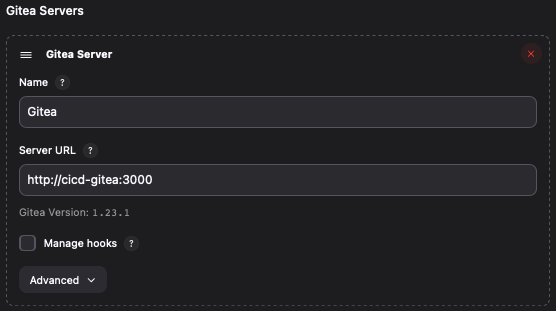
\includegraphics[width=.75\textwidth]{assets/gitea-servers}
\end{center}

\noindent Thereafter, a \verb|Gitea| Jenkins item was created. In its configuration section,
the repository sources were configured to point at the aforementioned \verb|CICD|
organisation. This is also where the access token of the \verb|jenkins| user was
supplied.

\begin{center}
	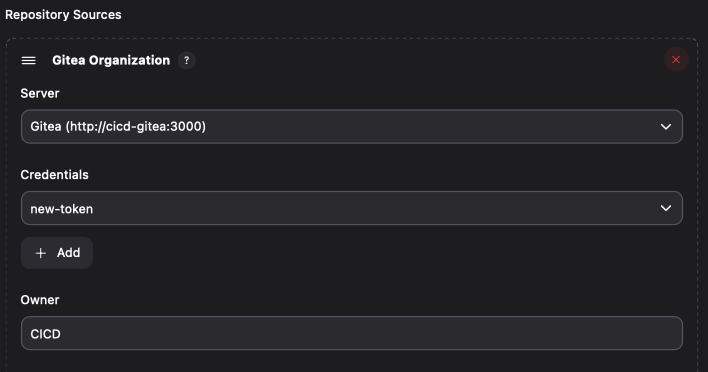
\includegraphics[width=.75\textwidth]{assets/repo-sources}
\end{center}

\noindent This configuration allows Jenkins to detect changes on Gitea repositories in the
designated organisation. Although this config does the job just fine, and lets
the Jenkins instance build codebases through the included \verb|Jenskinsfile|s,
it does not allow us to specify a custom (dockerized) environment for each build.
To change this, the \textbf{Docker plugin} and the \textbf{Docker pipeline}
plugins were installed. This, together with the previous docker-level configuration
of the Jenkins container, allows it to instantiate a new container for each build.
This way, the developer may specify a prefered docker image that is shipped with the
required build environment, such as the one needed to, among others, build a \textit{Spring Boot}
application $\dots$
\begin{lstlisting}
...
pipeline {
    agent {
        docker {
            image 'openjdk:17-slim'
            args '--network=bap_cicd'
        }
    }
    ...
\end{lstlisting}
\section{Reposilite}
The artifact repository, \textbf{Reposilite}, came with what was by far the least
convoluted setup procedure. In fact, it on its own did not require any configuration
whatsoever.\\
Setting up \textbf{Gradle} to publish artifacts to reposilite's \textit{releases} repo
included setting up a publication as follows:
\begin{lstlisting}
publishing {
    publications {
        create<MavenPublication>("reposilitePublication") {
            from(components["kotlin"])
        }
    }
    repositories {
        maven {
            url = uri("http://reposilite:8080/releases")
            credentials {
                isAllowInsecureProtocol = true
                username = "admin"
                password = "secret"
            }
        }
    }
}
\end{lstlisting}
Note that we need to explicitly allow the use of HTTP (instead of HTTPS) through \verb|isAllowInsecureProtocol|.
This gradle target is then invoked as the last step of the Jenkins pipeline:
\begin{lstlisting}
...
stages {
    stage('Build') {
        ...
    }

    stage('Publish Artifacts') {
        steps {
            script {
                sh "./gradlew publish"
            }
        }
    }
}
\end{lstlisting}
Upon invoking the pipeline, the artifacts become available in the repository:
\begin{center}
	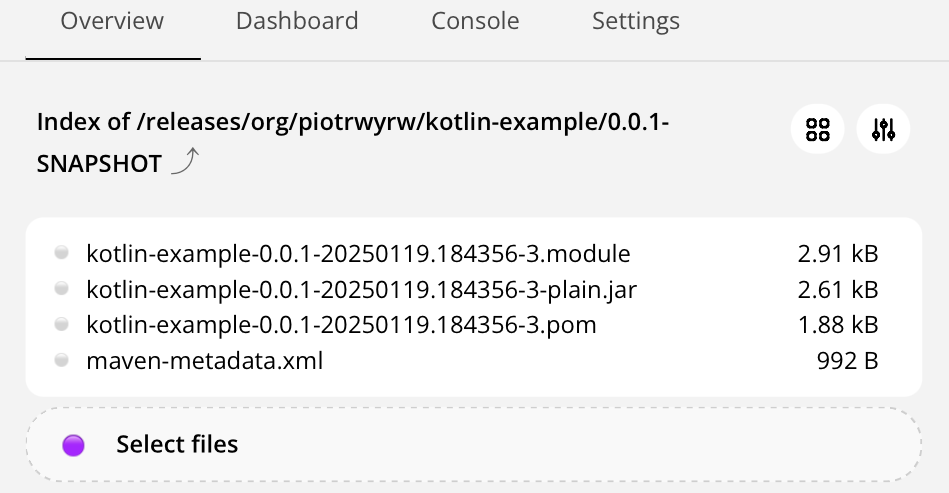
\includegraphics[width=.75\textwidth]{assets/artifacts}
\end{center}
